\section{METODOLOGI}

% Ubah konten-konten berikut sesuai dengan isi dari metodologi

\subsection{Metode yang digunakan}

Pada penelitian ini nantinya akan terdiri dari 2 langkah utama yaitu perancangan pada perangkat lunak (Softrware) dan perancangan pada perangkat keras (Hardware) :
%\begin{figure}[H]
%	\centering
%	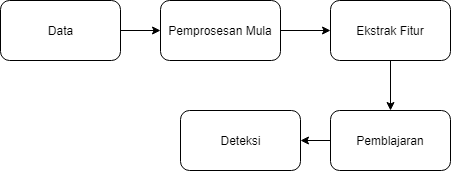
\includegraphics[width=\linewidth]{bab3/BlokDiagram}
%	\caption{Blok Diagram Penelitian}
%	\label{fig:blokdiagram}
%\end{figure}

\subsubsection{Perangkat Lunak}
Pada tahap ini akan dilakukan metode untuk membuat kendali pada mobil robot pada sisi perangkat lunak. Perangkat lunak ini akan dimulai dari pembuatan dataset dilanjutkan ke pose. Setelah pose akan dilanjutkan kepada tahapan klasifikasi dimana pada tahapan ini akan dilakukan pembelajaran mesin untuk dapat mengenali pose yang diberikan. Setelah tahap klasifikasi akan dilakukan tahap pembuatan program pada robot untuk dapat memahami data yang diterima dari tahap klasifikasi.

\begin{figure}[!h]
	\centering
	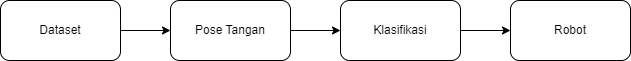
\includegraphics[width=1\linewidth]{gambar/gambar3.1}
	\caption{Blok Diagram Perangkat Lunak}
	\label{fig:gambar31}
\end{figure}

\begin{enumerate}
  \item Dataset \par
  Pada tahapan dataset disini akan dilakukan mulai dari pengambilan data-data yang disini nantinya akan berupa gambar/citra sampai dengan menyeleksi citra tersebut dan siap melanjutkan ke tahapan selanjutnya.

\begin{figure}[!h]
	\centering
	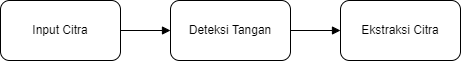
\includegraphics[width=0.7\linewidth]{gambar/Dataset.png}
	\caption{Blok Diagram Pembuatan Dataset}
	\label{fig:gambar32}
\end{figure}

\begin{enumerate}
  \item Input Citra \par
  Pada dasarnya untuk mendeteksi suatu pose atau gerakan dari tangan membutuhkan untuk menemukan bagian tangan pada setiap Frame dan kemudian menganalisa pose atau gerakan tangan tersebut. Kamera digunakan untuk mendapatkan pose dari tangan pada setiap frame yang akan digunakan oleh user sebagai input untuk menentukan perintah. Dari input kamera ini yang nantinya akan digunakan untuk mendeteksi adanya tangan pada frame menggunakan Mediapipe.
  \item Deteksi Tangan \par
  %Mediapipe pada tangan memiliki 21 titik keypoint pada tangan. Setiap keypoint memiliki atribut posisi x, y, dan z. Data dari setiap titik yang nantinya akan diolah untuk menentukan gerakan dari tangan. Data koordinat dari setiap keypoint yang telah di dapatkan akan dilakukan normalisasi. Koordinat yang telah didapatkan merupakan koordinat dari setiap titik terhadap titik nol citra. Maka diperlukan perubahan dimana  koordinat setiap titik dirubah menjadi terhadap titik 0 keypoint. Jadi setiap ada perubahan posisi pada tangan masih dapat terukur posisinya terhadap titik 0 keypoint. Untuk jarak antar keypoint akan di scaling menggunakan jarak titik 0 ke titik 5 untuk menangani masalah dekat atau jauhnya tangan dari kamera. Untuk sudut pada tangan akan ada 3 titik dimana dianggap tidak bisa berotasi atau memilki sudut 0° yaitu pada titik 0, 5, dan 17. Dari titik - titik yang diketahui akan dihubungkan hingga berbentuk rangka dari tangan. Dari koordinat pada setiap titik tersebut akan dicari nilai terkecil terhadap sumbu x dan sumbu y pada citra. Dari nilai terkecil tersebut akan dibuatkan sebuah kotak untuk menandai bahwa yang didalam kotak tersebut adalah rangka tangan yang telah terdeteksi oleh mediapipe. 
  Untuk mendeteksi tangan pada frame-frame yang telah ditangkap oleh kamera akan digunakan \textit{framework} Mediapipe. Mendeteksi tangan akan dimulai dari mendeteksi telapak tangan yang disebut sebagai \textit{palm detection model}. Setelah melakukan pendeteksian telapak tangan pada keseluruhan gambar maka berikutnya yaitu mendeteksi 21 titik \textit{keypoint} dalam wilayah tangan menggunakan regresi. Setelah 21 titik \textit{keypoint} terdeteksi maka langkah selanjutnya yaitu menghubungkan titik-titik yang telah terdeteksi sehingga dapat membentuk seperti rangka tangan yang ditunjukkan oleh Gambar \ref*{fig:tangan}.

  \item Ekstraksi Citra \par
  Tangan yang telah terdeteksi oleh mediapipe dan telah terdapat rangkanya pada setiap frame akan disimpan untuk menjadi dataset. Citra yang disimpan akan ada 2 macam yaitu citra yang ditangkap oleh kamera dan terdapat ditangannya dan juga terdapat citra dengan latar berwarna hitam dengan rangka tangan dari mediapipe didalamnya. Citra berwana hitam sebelum disimpan akan dipotong sesuai luas dari kotak yang diambil dari koordinat terkecil dari 21 titik mediapipe. Ukuran dari citra yang telah dipotong akan diubah menjadi 128 {\textit{pixels}} secara vertikal dan 128 {\textit{pixels}} secara horizontal. Setelah ukuran citra hitam ini diubah menjadi 128 $\times$ 128 {\textit{pixels}}, citra tersebut akan disimpan dalam bentuk file png.
\end{enumerate}

  \item Pose tangan \par
  Gestur tangan yang akan digunakan nantinya akan ada 5 getur yang akan sebagai simbol dari diam, maju, mundur, belok kanan, dan belok kiri. Diam akan disimbolkan dengan membuka telapak tangan serta meluruskan semua jari tangan. Maju akan disimbolkan dengan tangan mengepal. Mundur akan disimbolkan dengan meluruskan jari telunjuk, tengah, dan manis namun mengepalkan ibu jari dan jari kelingking. Belok kanan akan disimbolkan dengan meluruskan ibu jari dan mengepalkan semua jari kecuali ibu jari. Belok kiri akan disimbolkan dengan meluruskan jari kelingking dan mengepalkan semua jari kecuali jari kelingking.
  
  \item Klasifikasi \par
  Data yang sudah didapatkan nantinya akan di inputkan ke dalam perhitungan menggunakan machine learning. Data yang telah diinputkan nantinya akan dilabeli untuk ada diklasifikasikan dan digunakan untuk memberikan action selanjutnya. Dari hasil kalsifikasi nantinya akan disimpan sebagai model yang nantinya akan digunakan untuk mendeteksi citra yang akan datang
  
  \item Robot \par
  Dari data yang telah di klasifikasikan dan sudah didapatkan gesturnya maka gestur tersebut akan diterjemahkan ke dalam suatu perintah untuk dapat menggerakkan mobil robot. Robot akan menerima data dari hasil klasifikasi dan selanjutnya akan bergerak sesuai data yang diberikan. Gerakan robot akan diatur melalui arah dan kecepatan putaran pada roda. Robot akan berjalan maju jikalau arah dan kecepatan putaran roda bernilai sama dan akan berbelok bilah salah satu dari arah dan kecepatan putaran berbeda.
\end{enumerate}

\subsubsection{Perangkat Keras}
Pada tahap ini akan dilakukan metode untuk membuat kendali pada robot dari sisi pernagkat keras. Perangkat yang akan digunakan yaitu Laptop, modul \textit{bluetooth}, dan robot. 
\begin{figure}[!h]
	\centering
	\includegraphics[width=0.7\linewidth]{"gambar/gambar perangkat keras"}
	\caption{Blok Diagram Perangkat Keras}
	\label{fig:gambar33}
\end{figure}

\begin{enumerate}
  \item Laptop \par
  Laptop disini nantinya akan digunakan untuk menjalankan program perangkat lunak yang telah dikembangnkan untuk dapat menklasifikasikan tangan yang terdeteksi dan juga kamera yang terdapat pada laptop ini juga yang nantinya akan digunakan sebagai input gambar/citra.

  \item \textit{Bluetooth} \par
  Hasil klasifikasi yang ada pada laptop akan dikirim ke mobil robot untuk dapat memberikannya perintah sesuia dari hasil klasifikasi. Menghubungkan laptop dan robot ini akan menggunakan modul \textit{bluetooth} yang akan dihubungkan dengan mobil robot dikarenakan mobil robot yang akan digunakan masih belum mempunyai modul \textit{bluetooth}. 

  \item Robot \par
  Pada bagian mobil robot ini terdapat beberapa komponen elektronik yang terpasang, diantaranya sebuatu mikrokontroller Arduino uno dan mikrokontroller Arduino nano , 2 buah .FC-03 L298N motor driver dual, modul charger Tp 4056, dan modul bluetooth HC-05. Komponen mekanik terdapat 4 buah roda, 4 buah gearbox motor, dan 1 buah chassis.
\end{enumerate}

\subsection{Urutan pelaksanaan penelitian}

% Ubah tabel berikut sesuai dengan isi dari rencana kerja
\begin{table}[!h]
  \caption{Urutan pelaksanaan penelitian}
  \begin{tabular}{|c|cccccccccccccccc}
  \hline
                                                                                & \multicolumn{16}{c|}{Minggu}                                                                                                                                                                                                                                                                                                                                                                                         \\ \cline{2-17} 
  \multirow{-2}{*}{Kegiatan}                                                    & \multicolumn{1}{c|}{1} & \multicolumn{1}{c|}{2} & \multicolumn{1}{c|}{3} & \multicolumn{1}{c|}{4} & \multicolumn{1}{c|}{5} & \multicolumn{1}{c|}{6} & \multicolumn{1}{c|}{7} & \multicolumn{1}{c|}{8} & \multicolumn{1}{c|}{9} & \multicolumn{1}{c|}{10} & \multicolumn{1}{c|}{11} & \multicolumn{1}{c|}{12} & \multicolumn{1}{c|}{13} & \multicolumn{1}{c|}{14} & \multicolumn{1}{c|}{15} & \multicolumn{1}{c|}{16} \\ \hline
  \begin{tabular}[c]{@{}c@{}}Pengambilan dan \\ pemrosesan dataset\end{tabular} & \multicolumn{3}{c|}{\cellcolor[HTML]{656565}}                            & \multicolumn{1}{c|}{}  & \multicolumn{1}{c|}{}  & \multicolumn{1}{c|}{}  & \multicolumn{1}{c|}{}  & \multicolumn{1}{c|}{}  & \multicolumn{1}{c|}{}  & \multicolumn{1}{c|}{}   & \multicolumn{1}{c|}{}   & \multicolumn{1}{c|}{}   & \multicolumn{1}{c|}{}   & \multicolumn{1}{c|}{}   & \multicolumn{1}{c|}{}   & \multicolumn{1}{c|}{}   \\ \hline
  Klasifikasi                                                                   & \multicolumn{1}{l|}{}  & \multicolumn{1}{l|}{}  & \multicolumn{1}{l|}{}  & \multicolumn{5}{l|}{\cellcolor[HTML]{656565}}                                                                              & \multicolumn{1}{l|}{}  & \multicolumn{1}{l|}{}   & \multicolumn{1}{l|}{}   & \multicolumn{1}{l|}{}   & \multicolumn{1}{l|}{}   & \multicolumn{1}{l|}{}   & \multicolumn{1}{l|}{}   & \multicolumn{1}{l|}{}   \\ \hline
  Perakitan mobil robot                                                         & \multicolumn{1}{c|}{}  & \multicolumn{1}{c|}{}  & \multicolumn{1}{c|}{}  & \multicolumn{1}{c|}{}  & \multicolumn{1}{c|}{}  & \multicolumn{1}{c|}{}  & \multicolumn{1}{c|}{}  & \multicolumn{1}{c|}{}  & \multicolumn{2}{c|}{\cellcolor[HTML]{656565}}    & \multicolumn{1}{c|}{}   & \multicolumn{1}{c|}{}   & \multicolumn{1}{c|}{}   & \multicolumn{1}{c|}{}   & \multicolumn{1}{c|}{}   & \multicolumn{1}{c|}{}   \\ \hline
  \begin{tabular}[c]{@{}c@{}}Pembuatan program \\ gerakan mobil\end{tabular}    & \multicolumn{1}{c|}{}  & \multicolumn{1}{c|}{}  & \multicolumn{1}{c|}{}  & \multicolumn{1}{c|}{}  & \multicolumn{1}{c|}{}  & \multicolumn{1}{c|}{}  & \multicolumn{1}{c|}{}  & \multicolumn{1}{c|}{}  & \multicolumn{1}{c|}{}  & \multicolumn{1}{c|}{}   & \multicolumn{3}{c|}{\cellcolor[HTML]{656565}}                               & \multicolumn{1}{c|}{}   & \multicolumn{1}{c|}{}   & \multicolumn{1}{c|}{}   \\ \hline
  \multicolumn{1}{|l|}{Pengujian dan analisa}                                   & \multicolumn{1}{l|}{}  & \multicolumn{1}{l|}{}  & \multicolumn{1}{l|}{}  & \multicolumn{1}{l|}{}  & \multicolumn{1}{l|}{}  & \multicolumn{1}{l|}{}  & \multicolumn{1}{l|}{}  & \multicolumn{1}{l|}{}  & \multicolumn{1}{l|}{}  & \multicolumn{1}{l|}{}   & \multicolumn{1}{l|}{}   & \multicolumn{1}{l|}{}   & \multicolumn{1}{l|}{}   & \multicolumn{3}{l}{\cellcolor[HTML]{656565}{\color[HTML]{656565} }}         \\ \hline
  \end{tabular}
  \end{table}
